% Options for packages loaded elsewhere
\PassOptionsToPackage{unicode}{hyperref}
\PassOptionsToPackage{hyphens}{url}
%
\documentclass[
]{article}
\usepackage{lmodern}
\usepackage{amssymb,amsmath}
\usepackage{ifxetex,ifluatex}
\ifnum 0\ifxetex 1\fi\ifluatex 1\fi=0 % if pdftex
  \usepackage[T1]{fontenc}
  \usepackage[utf8]{inputenc}
  \usepackage{textcomp} % provide euro and other symbols
\else % if luatex or xetex
  \usepackage{unicode-math}
  \defaultfontfeatures{Scale=MatchLowercase}
  \defaultfontfeatures[\rmfamily]{Ligatures=TeX,Scale=1}
\fi
% Use upquote if available, for straight quotes in verbatim environments
\IfFileExists{upquote.sty}{\usepackage{upquote}}{}
\IfFileExists{microtype.sty}{% use microtype if available
  \usepackage[]{microtype}
  \UseMicrotypeSet[protrusion]{basicmath} % disable protrusion for tt fonts
}{}
\makeatletter
\@ifundefined{KOMAClassName}{% if non-KOMA class
  \IfFileExists{parskip.sty}{%
    \usepackage{parskip}
  }{% else
    \setlength{\parindent}{0pt}
    \setlength{\parskip}{6pt plus 2pt minus 1pt}}
}{% if KOMA class
  \KOMAoptions{parskip=half}}
\makeatother
\usepackage{xcolor}
\IfFileExists{xurl.sty}{\usepackage{xurl}}{} % add URL line breaks if available
\IfFileExists{bookmark.sty}{\usepackage{bookmark}}{\usepackage{hyperref}}
\hypersetup{
  pdftitle={R Notebook},
  hidelinks,
  pdfcreator={LaTeX via pandoc}}
\urlstyle{same} % disable monospaced font for URLs
\usepackage[margin=1in]{geometry}
\usepackage{color}
\usepackage{fancyvrb}
\newcommand{\VerbBar}{|}
\newcommand{\VERB}{\Verb[commandchars=\\\{\}]}
\DefineVerbatimEnvironment{Highlighting}{Verbatim}{commandchars=\\\{\}}
% Add ',fontsize=\small' for more characters per line
\usepackage{framed}
\definecolor{shadecolor}{RGB}{248,248,248}
\newenvironment{Shaded}{\begin{snugshade}}{\end{snugshade}}
\newcommand{\AlertTok}[1]{\textcolor[rgb]{0.94,0.16,0.16}{#1}}
\newcommand{\AnnotationTok}[1]{\textcolor[rgb]{0.56,0.35,0.01}{\textbf{\textit{#1}}}}
\newcommand{\AttributeTok}[1]{\textcolor[rgb]{0.77,0.63,0.00}{#1}}
\newcommand{\BaseNTok}[1]{\textcolor[rgb]{0.00,0.00,0.81}{#1}}
\newcommand{\BuiltInTok}[1]{#1}
\newcommand{\CharTok}[1]{\textcolor[rgb]{0.31,0.60,0.02}{#1}}
\newcommand{\CommentTok}[1]{\textcolor[rgb]{0.56,0.35,0.01}{\textit{#1}}}
\newcommand{\CommentVarTok}[1]{\textcolor[rgb]{0.56,0.35,0.01}{\textbf{\textit{#1}}}}
\newcommand{\ConstantTok}[1]{\textcolor[rgb]{0.00,0.00,0.00}{#1}}
\newcommand{\ControlFlowTok}[1]{\textcolor[rgb]{0.13,0.29,0.53}{\textbf{#1}}}
\newcommand{\DataTypeTok}[1]{\textcolor[rgb]{0.13,0.29,0.53}{#1}}
\newcommand{\DecValTok}[1]{\textcolor[rgb]{0.00,0.00,0.81}{#1}}
\newcommand{\DocumentationTok}[1]{\textcolor[rgb]{0.56,0.35,0.01}{\textbf{\textit{#1}}}}
\newcommand{\ErrorTok}[1]{\textcolor[rgb]{0.64,0.00,0.00}{\textbf{#1}}}
\newcommand{\ExtensionTok}[1]{#1}
\newcommand{\FloatTok}[1]{\textcolor[rgb]{0.00,0.00,0.81}{#1}}
\newcommand{\FunctionTok}[1]{\textcolor[rgb]{0.00,0.00,0.00}{#1}}
\newcommand{\ImportTok}[1]{#1}
\newcommand{\InformationTok}[1]{\textcolor[rgb]{0.56,0.35,0.01}{\textbf{\textit{#1}}}}
\newcommand{\KeywordTok}[1]{\textcolor[rgb]{0.13,0.29,0.53}{\textbf{#1}}}
\newcommand{\NormalTok}[1]{#1}
\newcommand{\OperatorTok}[1]{\textcolor[rgb]{0.81,0.36,0.00}{\textbf{#1}}}
\newcommand{\OtherTok}[1]{\textcolor[rgb]{0.56,0.35,0.01}{#1}}
\newcommand{\PreprocessorTok}[1]{\textcolor[rgb]{0.56,0.35,0.01}{\textit{#1}}}
\newcommand{\RegionMarkerTok}[1]{#1}
\newcommand{\SpecialCharTok}[1]{\textcolor[rgb]{0.00,0.00,0.00}{#1}}
\newcommand{\SpecialStringTok}[1]{\textcolor[rgb]{0.31,0.60,0.02}{#1}}
\newcommand{\StringTok}[1]{\textcolor[rgb]{0.31,0.60,0.02}{#1}}
\newcommand{\VariableTok}[1]{\textcolor[rgb]{0.00,0.00,0.00}{#1}}
\newcommand{\VerbatimStringTok}[1]{\textcolor[rgb]{0.31,0.60,0.02}{#1}}
\newcommand{\WarningTok}[1]{\textcolor[rgb]{0.56,0.35,0.01}{\textbf{\textit{#1}}}}
\usepackage{graphicx}
\makeatletter
\def\maxwidth{\ifdim\Gin@nat@width>\linewidth\linewidth\else\Gin@nat@width\fi}
\def\maxheight{\ifdim\Gin@nat@height>\textheight\textheight\else\Gin@nat@height\fi}
\makeatother
% Scale images if necessary, so that they will not overflow the page
% margins by default, and it is still possible to overwrite the defaults
% using explicit options in \includegraphics[width, height, ...]{}
\setkeys{Gin}{width=\maxwidth,height=\maxheight,keepaspectratio}
% Set default figure placement to htbp
\makeatletter
\def\fps@figure{htbp}
\makeatother
\setlength{\emergencystretch}{3em} % prevent overfull lines
\providecommand{\tightlist}{%
  \setlength{\itemsep}{0pt}\setlength{\parskip}{0pt}}
\setcounter{secnumdepth}{-\maxdimen} % remove section numbering
\newcommand{\R}{\textnormal{\sffamily\bfseries R}}}
\usepackage{booktabs}
\usepackage{longtable}
\usepackage{array}
\usepackage{multirow}
\usepackage{wrapfig}
\usepackage{float}
\usepackage{colortbl}
\usepackage{pdflscape}
\usepackage{tabu}
\usepackage{threeparttable}
\usepackage{threeparttablex}
\usepackage[normalem]{ulem}
\usepackage{makecell}
\usepackage{xcolor}
\ifluatex
  \usepackage{selnolig}  % disable illegal ligatures
\fi

\title{R Notebook}
\author{}
\date{\vspace{-2.5em}}

\begin{document}
\maketitle

\textbf{Implementation}

In this section we present a practical illustration of the algorithms
discussed. For the sake of simplicity we use a random walk plus noise
model, i.e.~the most basic form of a linear Gaussian state-space model.
\begin{align}
y_{t}|x_{t} & \sim N(x_{t},\sigma^{2}) \\
x_{t}|x_{t-1} & \sim N(x_{t-1},\tau^{2}) \\
x_{0} & \sim N(m_{0},C_{0})
\end{align} As already mentioned before, in this case the filtering
distribution can be computed in closed form solutions using the Kalman
filter. However, this toy example will be used also to illustrate more
involving filtering strategies described in this work. We believe indeed
that it represents a useful starting point to understand the logic of
the algorithms which may be eventually replicated when dealing with more
complex models.\\
The filtering strategy is applied to 50 simulated data. Figure XX shows
the simulated true states sequence assuming as data generating process
the Equation (2) with \(\tau^{2}=1\) and simulated observed sequence
process form Equation (1) with \(\sigma^{2}=1\).

\begin{figure}[ht]

{\centering \includegraphics{Exemples-and-Implementations_files/figure-latex/unnamed-chunk-3-1} 

}

\caption{Simulated random walk plus noise model}\label{fig:unnamed-chunk-3}
\end{figure}

The Kalman Filter for this model is implemented as described below.

\begin{itemize}
\item Initialize $\theta_{0} \sim N(m_{0},C_{0})$
\item For $t=1,..N$
\begin{enumerate}
\item Compute the one-step-ahead state predictive distribution at time $t-1$
\begin{align*}
x_{t}|y_{1:t-1} & \sim N(a_{t},R_{t})\\
a_{t} & = m_{t-1}\\
R_{t} & = C_{t-1}+\tau^2
\end{align*}
\item Compute the filtering distribution at time $t$ as $p(x_{t}|y_{1:t}) \propto p(x_{t}|y_{1:t-1})p(y_{t}|x_{t})$, i.e. the product of the one-step-ahead state predictive distribution and the likelihood
\begin{align*}
x_{t}|y_{1:t} & \sim N(m_{t},C_{t}) \\
m_{t} & = \big(1-\frac{R_{t}}{R_{t}+\sigma^2}\big)a_{t}+\frac{R_{t}}{R_{t}+\sigma^2}y_{t} \\
C_{t} & = \frac{R_{t}}{R_{t}+\sigma^2}\sigma^2
\end{align*}
\end{enumerate}
\end{itemize}

These steps are summarize in the

\begin{Shaded}
\begin{Highlighting}[]
\NormalTok{DLM}\OtherTok{\textless{}{-}}\ControlFlowTok{function}\NormalTok{(data,sig2,tau2,m0,C0)\{}
\NormalTok{  n  }\OtherTok{=} \FunctionTok{length}\NormalTok{(data)}
\NormalTok{  m  }\OtherTok{=} \FunctionTok{rep}\NormalTok{(}\DecValTok{0}\NormalTok{,n)}
\NormalTok{  C  }\OtherTok{=} \FunctionTok{rep}\NormalTok{(}\DecValTok{0}\NormalTok{,n)}
  \ControlFlowTok{for}\NormalTok{ (t }\ControlFlowTok{in} \DecValTok{1}\SpecialCharTok{:}\NormalTok{n)\{}
    \ControlFlowTok{if}\NormalTok{ (t}\SpecialCharTok{==}\DecValTok{1}\NormalTok{)\{}
\NormalTok{      a }\OtherTok{=}\NormalTok{ m0}
\NormalTok{      R }\OtherTok{=}\NormalTok{ C0 }\SpecialCharTok{+}\NormalTok{ tau2}
\NormalTok{    \}}\ControlFlowTok{else}\NormalTok{\{}
\NormalTok{      a }\OtherTok{=}\NormalTok{ m[t}\DecValTok{{-}1}\NormalTok{]}
\NormalTok{      R }\OtherTok{=}\NormalTok{ C[t}\DecValTok{{-}1}\NormalTok{] }\SpecialCharTok{+}\NormalTok{ tau2}
\NormalTok{    \}}
\NormalTok{    A }\OtherTok{=}\NormalTok{ R}\SpecialCharTok{/}\NormalTok{(R}\SpecialCharTok{+}\NormalTok{sig2)}
\NormalTok{    m[t] }\OtherTok{=}\NormalTok{ (}\DecValTok{1}\SpecialCharTok{{-}}\NormalTok{A)}\SpecialCharTok{*}\NormalTok{a }\SpecialCharTok{+}\NormalTok{ A}\SpecialCharTok{*}\NormalTok{y[t]}
\NormalTok{    C[t] }\OtherTok{=}\NormalTok{ A}\SpecialCharTok{*}\NormalTok{sig2}
\NormalTok{  \}}
  \FunctionTok{return}\NormalTok{(}\FunctionTok{list}\NormalTok{(}\AttributeTok{m=}\NormalTok{m,}\AttributeTok{C=}\NormalTok{C))}
\NormalTok{\}}
\end{Highlighting}
\end{Shaded}

In the Figure below we show the filtered states states estimated using
Kalman Filter with \(x_{0} \sim N(0,100)\) and
\(\sigma^{2}=\tau^{2}=1\). The filtered states follow the observations
closely and they provide a good approximation of the true states.

\begin{figure}[ht]

{\centering 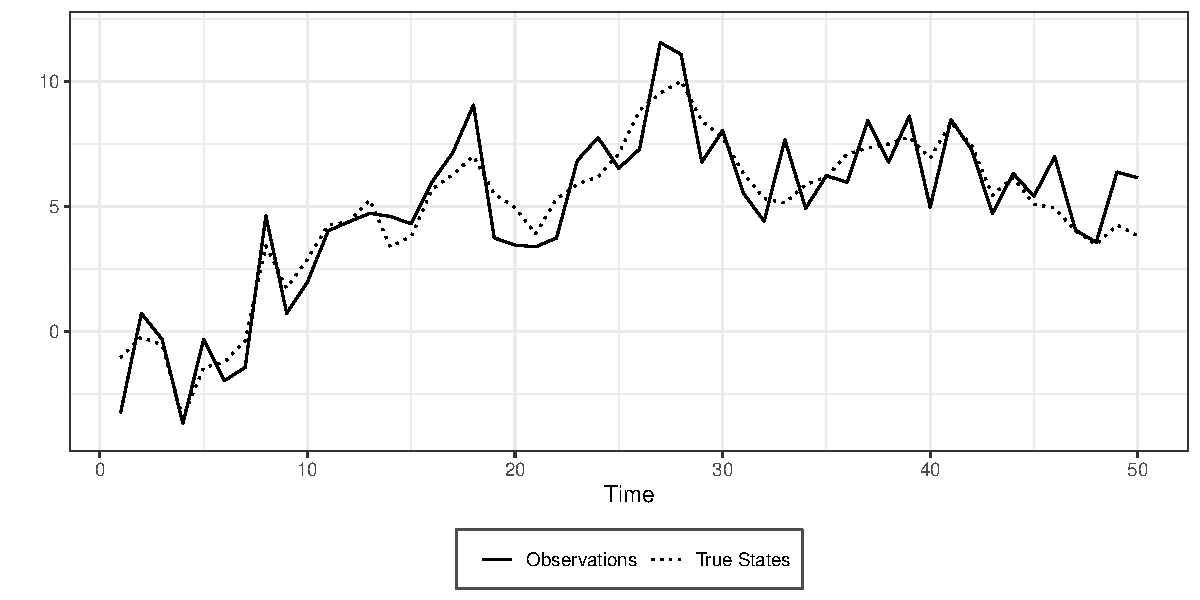
\includegraphics{Exemples-and-Implementations_files/figure-latex/unnamed-chunk-5-1} 

}

\caption{Kalman Filtered States with credible interval (in red)}\label{fig:unnamed-chunk-5}
\end{figure}

\textbf{Implementation} With reference to the random walk plus noise of
section XX, let \(\{(x_{0},w_{0})^{(i)}\}_{i=1}^{N}\) summarizes
\(p(x_{0}|y_{0})\) such that, for example,
\(E(g(x_{0})|y_{0}) \approx \frac{1}{N}\sum_{i=1}^{N}w_{0}^{(i)}g(x_{0}^{(i)})\).
For \(t=1,...,n\) where \(n\) is the length of the sample, at any
iteration

\begin{itemize}
\item Draw $x_{t}^{(i)} \sim N(x_{t-1}^{(i)},\tau^2) \ \ i=1,...,N$ such that $\{(x_{t},w_{t-1})^{(i)}\}_{i=1}^{N}$ summarizes $p(x_{t}|y_{t-1})$
\item Set $w_{t}^{(i)} = w_{t-1}^{(i)}f_{N}(y_{t};x_{t}^{(i)},\sigma^2) \ \ i=1,...,N$ such that $\{(x_{t},w_{t})^{(i)}\}_{i=1}^{N}$ summarizes $p(x_{t}|y_{t})$
\end{itemize}

\begin{Shaded}
\begin{Highlighting}[]
\NormalTok{SISfun}\OtherTok{\textless{}{-}}\ControlFlowTok{function}\NormalTok{(data,N,m0,C0,tau,sigma)\{}
\NormalTok{  xs}\OtherTok{\textless{}{-}}\ConstantTok{NULL}
\NormalTok{  ws}\OtherTok{\textless{}{-}}\ConstantTok{NULL}
\NormalTok{  ess}\OtherTok{\textless{}{-}}\ConstantTok{NULL}
\NormalTok{  x  }\OtherTok{=} \FunctionTok{rnorm}\NormalTok{(N,m0,}\FunctionTok{sqrt}\NormalTok{(C0))}
\NormalTok{  w  }\OtherTok{=} \FunctionTok{rep}\NormalTok{(}\DecValTok{1}\SpecialCharTok{/}\NormalTok{N,N)}
  \ControlFlowTok{for}\NormalTok{(t }\ControlFlowTok{in} \DecValTok{1}\SpecialCharTok{:}\FunctionTok{length}\NormalTok{(data))\{}
\NormalTok{    x    }\OtherTok{=} \FunctionTok{rnorm}\NormalTok{(N,x,tau)                   }\CommentTok{\#sample from N(x\_\{t{-}1\},tau)}
\NormalTok{    w    }\OtherTok{=}\NormalTok{ w}\SpecialCharTok{*}\FunctionTok{dnorm}\NormalTok{(data[t],x,sigma)         }\CommentTok{\#update weight}
\NormalTok{    xs }\OtherTok{=} \FunctionTok{rbind}\NormalTok{(xs,x)}
\NormalTok{    ws }\OtherTok{=} \FunctionTok{rbind}\NormalTok{(ws,w)}
    
\NormalTok{    wnorm}\OtherTok{=}\NormalTok{ w}\SpecialCharTok{/}\FunctionTok{sum}\NormalTok{(w)                         }\CommentTok{\#normalized weight}
\NormalTok{    ESS  }\OtherTok{=} \DecValTok{1}\SpecialCharTok{/}\FunctionTok{sum}\NormalTok{(wnorm}\SpecialCharTok{\^{}}\DecValTok{2}\NormalTok{)                   }\CommentTok{\#effective sample size}
    
\NormalTok{    ess }\OtherTok{=}\FunctionTok{rbind}\NormalTok{(ess,ESS)}
\NormalTok{  \}}
  
  \FunctionTok{return}\NormalTok{(}\FunctionTok{list}\NormalTok{(}\AttributeTok{xs=}\NormalTok{xs,}\AttributeTok{ws=}\NormalTok{ws,}\AttributeTok{ess=}\NormalTok{ess))}
\NormalTok{\}}
\end{Highlighting}
\end{Shaded}

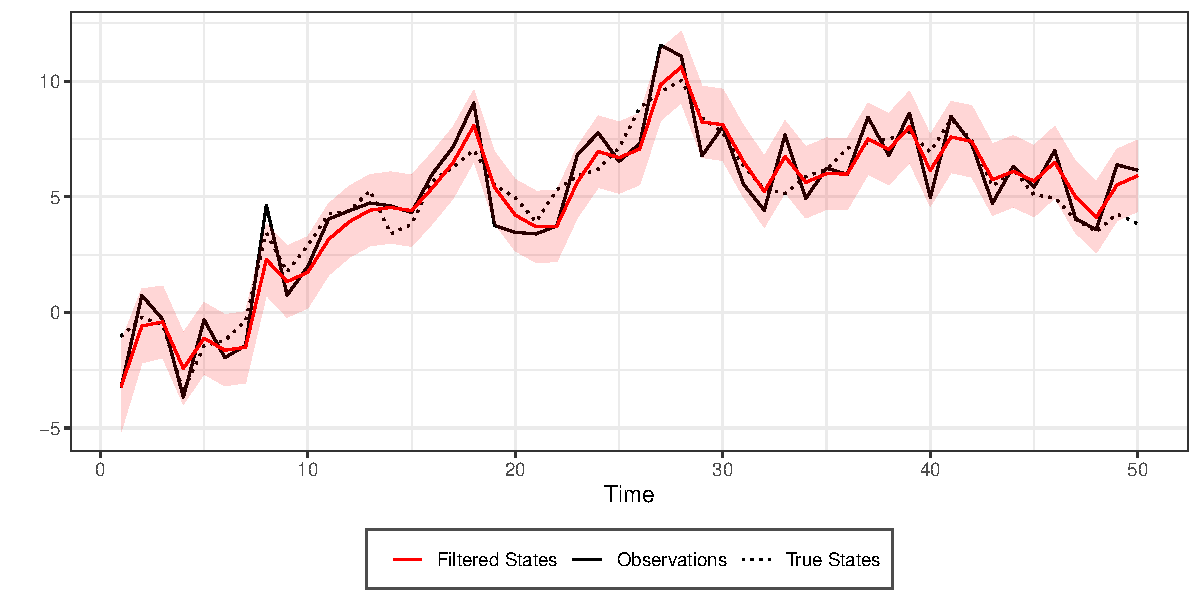
\includegraphics{Exemples-and-Implementations_files/figure-latex/unnamed-chunk-7-1.pdf}

\begin{figure}[ht]

{\centering 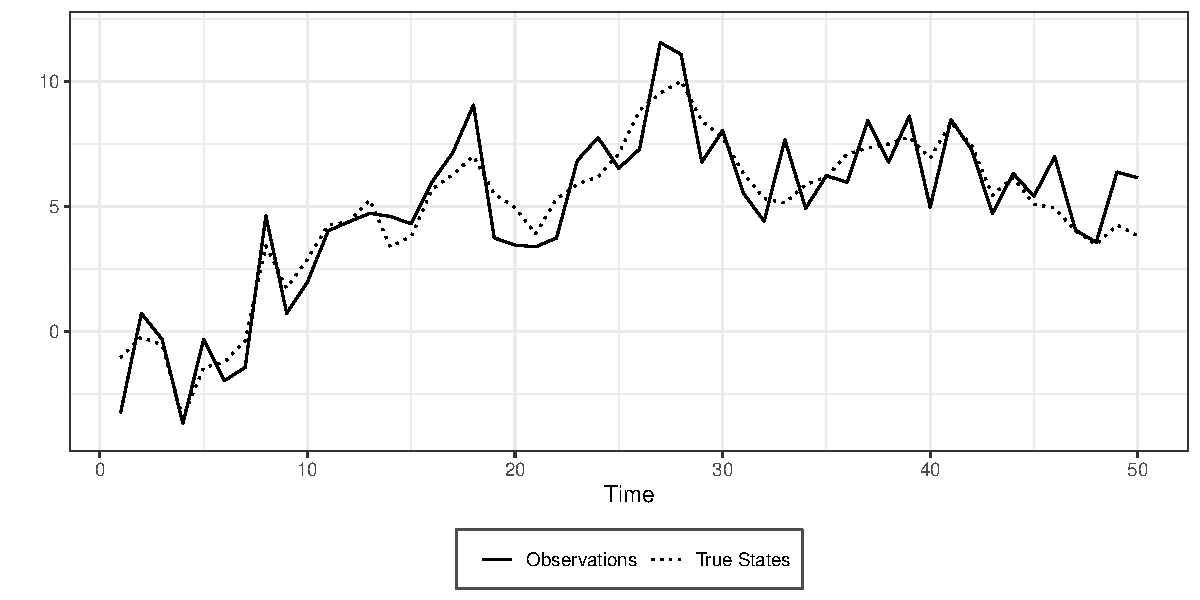
\includegraphics{Exemples-and-Implementations_files/figure-latex/unnamed-chunk-8-1} 

}

\caption{SIS Filtered States with credible interval (in red)}\label{fig:unnamed-chunk-8}
\end{figure}

\hfill\break
\textbf{Particle Filter}\\
With reference to the random walk plus noise of section XX, let
\(\{(x_{0},w_{0})^{(i)}\}_{i=1}^{N}\) summarizes \(p(x_{0}|y_{0})\) such
that, for example,
\(E(g(x_{0})|y_{0}) \approx \frac{1}{N}\sum_{i=1}^{N}w_{0}^{(i)}g(x_{0}^{(i)})\).
For \(t=1,...,n\) where \(n\) is the length of the sample, at any
iteration

\begin{itemize}
\item Draw $x_{t}^{(i)} \sim N(x_{t-1}^{(i)},\tau^2) \ \ i=1,...,N$ such that $\{(x_{t},w_{t-1})^{(i)}\}_{i=1}^{N}$ summarizes $p(x_{t}|y_{t-1})$
\item Set $w_{t}^{(i)} = w_{t-1}^{(i)}f_{N}(y_{t};x_{t}^{(i)},\sigma^2) \ \ i=1,...,N$ such that $\{(x_{t},w_{t})^{(i)}\}_{i=1}^{N}$ summarizes $p(x_{t}|y_{t})$
\end{itemize}

In addition, when \(ESS<ESS_{0}\)
\footnote{In our example we fix $ESS_{0}=N/2$, this is an arbitrary common rule of thumb.},
resempling applies

\begin{itemize}
\item Draw a sample of size N, $x_{t}^{(1)},...,x_{t}^{(N)}$,from the discrete distribution $P(x_{t}=x_{t}^{(i)})=w_{t}^{(i)},\ \ i=1,...,N$
\item Reset the weights: $w_{t}^{(i)}=N^{-1}$, $i=1,...,N$.
\end{itemize}

\begin{Shaded}
\begin{Highlighting}[]
\NormalTok{PFfun}\OtherTok{\textless{}{-}}\ControlFlowTok{function}\NormalTok{(data,N,m0,C0,tau,sigma,r)\{}
  \ControlFlowTok{if}\NormalTok{(}\FunctionTok{missing}\NormalTok{(r))\{r}\OtherTok{=}\DecValTok{2}\NormalTok{\}}\ControlFlowTok{else}\NormalTok{\{\}}
\NormalTok{  xs}\OtherTok{\textless{}{-}}\ConstantTok{NULL}
\NormalTok{  ws}\OtherTok{\textless{}{-}}\ConstantTok{NULL}
\NormalTok{  ess}\OtherTok{\textless{}{-}}\ConstantTok{NULL}
\NormalTok{  x  }\OtherTok{=} \FunctionTok{rnorm}\NormalTok{(N,m0,}\FunctionTok{sqrt}\NormalTok{(C0))}
\NormalTok{  w  }\OtherTok{=} \FunctionTok{rep}\NormalTok{(}\DecValTok{1}\SpecialCharTok{/}\NormalTok{N,N)}
   
  \ControlFlowTok{for}\NormalTok{(t }\ControlFlowTok{in} \DecValTok{1}\SpecialCharTok{:}\FunctionTok{length}\NormalTok{(data))\{}
    
\NormalTok{    x}\OtherTok{\textless{}{-}}\FunctionTok{rnorm}\NormalTok{(N,x,tau)}
\NormalTok{    w1}\OtherTok{\textless{}{-}}\NormalTok{w}\SpecialCharTok{*}\FunctionTok{dnorm}\NormalTok{(data[t],x,sigma)}
    
\NormalTok{    w }\OtherTok{=}\NormalTok{ w1}\SpecialCharTok{/}\FunctionTok{sum}\NormalTok{(w1)}
\NormalTok{    ESS  }\OtherTok{=} \DecValTok{1}\SpecialCharTok{/}\FunctionTok{sum}\NormalTok{(w}\SpecialCharTok{\^{}}\DecValTok{2}\NormalTok{)}
    
    \ControlFlowTok{if}\NormalTok{(ESS}\SpecialCharTok{\textless{}}\NormalTok{(N}\SpecialCharTok{/}\NormalTok{r))\{}
\NormalTok{      index}\OtherTok{\textless{}{-}}\FunctionTok{sample}\NormalTok{(N,}\AttributeTok{size=}\NormalTok{N,}\AttributeTok{replace=}\NormalTok{T,}\AttributeTok{prob=}\NormalTok{w)}
\NormalTok{      x}\OtherTok{\textless{}{-}}\NormalTok{x[index]}
\NormalTok{      w}\OtherTok{\textless{}{-}}\FunctionTok{rep}\NormalTok{(}\DecValTok{1}\SpecialCharTok{/}\NormalTok{N,N)}
\NormalTok{    \}}\ControlFlowTok{else}\NormalTok{\{\}}
    
\NormalTok{    xs }\OtherTok{=} \FunctionTok{rbind}\NormalTok{(xs,x)}
\NormalTok{    ws }\OtherTok{=} \FunctionTok{rbind}\NormalTok{(ws,w)}
\NormalTok{    ess }\OtherTok{=}\FunctionTok{rbind}\NormalTok{(ess,ESS)}
\NormalTok{  \}}
  \FunctionTok{return}\NormalTok{(}\FunctionTok{list}\NormalTok{(}\AttributeTok{xs=}\NormalTok{xs,}\AttributeTok{ws=}\NormalTok{ws,}\AttributeTok{ess=}\NormalTok{ess))}
\NormalTok{\}}
\end{Highlighting}
\end{Shaded}

\begin{figure}[ht]

{\centering 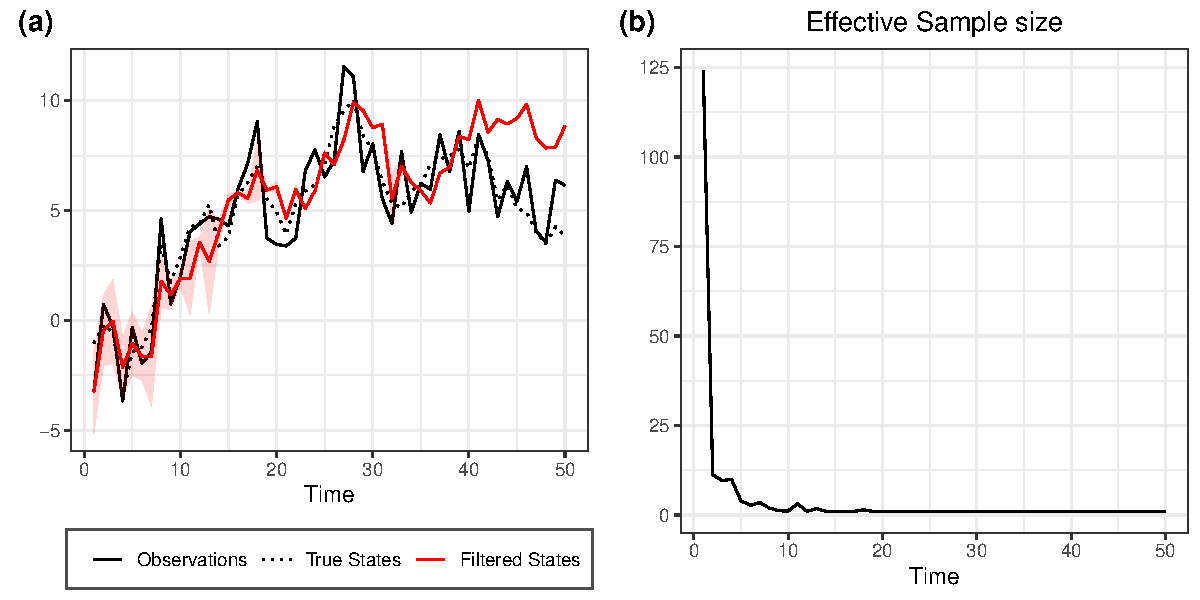
\includegraphics{Exemples-and-Implementations_files/figure-latex/unnamed-chunk-10-1} 

}

\caption{Effective Sample Size}\label{fig:unnamed-chunk-10}
\end{figure}

\begin{figure}[ht]

{\centering 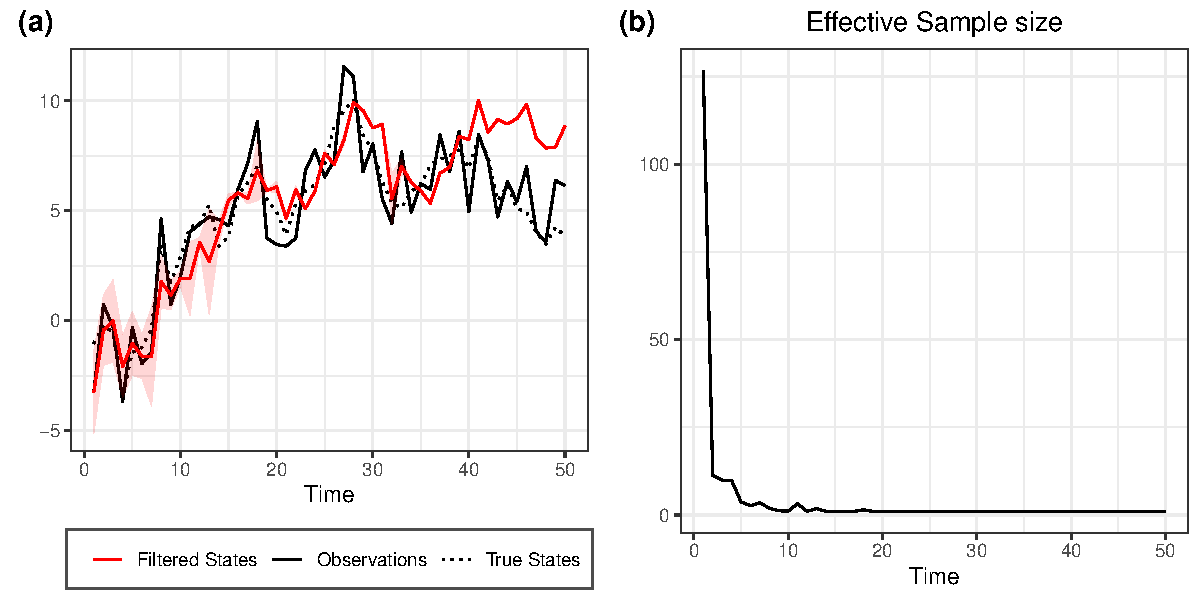
\includegraphics{Exemples-and-Implementations_files/figure-latex/unnamed-chunk-11-1} 

}

\caption{Particle Filtered States with credible interval (in red)}\label{fig:unnamed-chunk-11}
\end{figure}

\textbf{Particle Filter Petroni more efficient}

\begin{Shaded}
\begin{Highlighting}[]
\NormalTok{PF2fun}\OtherTok{\textless{}{-}}\ControlFlowTok{function}\NormalTok{(data,N,m0,C0,tau,sigma,r)\{}
  \ControlFlowTok{if}\NormalTok{(}\FunctionTok{missing}\NormalTok{(r))\{r}\OtherTok{=}\DecValTok{2}\NormalTok{\}}\ControlFlowTok{else}\NormalTok{\{\}}
\NormalTok{  xs}\OtherTok{\textless{}{-}}\ConstantTok{NULL}
\NormalTok{  ws}\OtherTok{\textless{}{-}}\ConstantTok{NULL}
\NormalTok{  ess}\OtherTok{\textless{}{-}}\ConstantTok{NULL}
\NormalTok{  x  }\OtherTok{=} \FunctionTok{rnorm}\NormalTok{(N,m0,}\FunctionTok{sqrt}\NormalTok{(C0))}
\NormalTok{  importancesd}\OtherTok{\textless{}{-}}\FunctionTok{sqrt}\NormalTok{(tau }\SpecialCharTok{{-}}\NormalTok{ tau}\SpecialCharTok{\^{}}\DecValTok{2} \SpecialCharTok{/}\NormalTok{(tau }\SpecialCharTok{+}\NormalTok{ sigma))}
\NormalTok{  predsd }\OtherTok{\textless{}{-}} \FunctionTok{sqrt}\NormalTok{(sigma}\SpecialCharTok{+}\NormalTok{tau)}
\NormalTok{  w  }\OtherTok{=} \FunctionTok{rep}\NormalTok{(}\DecValTok{1}\SpecialCharTok{/}\NormalTok{N,N)}
  
  \ControlFlowTok{for}\NormalTok{(t }\ControlFlowTok{in} \DecValTok{1}\SpecialCharTok{:}\FunctionTok{length}\NormalTok{(data))\{}
    
\NormalTok{    means}\OtherTok{\textless{}{-}}\NormalTok{x}\SpecialCharTok{+}\NormalTok{(tau}\SpecialCharTok{/}\NormalTok{(tau}\SpecialCharTok{+}\NormalTok{sigma))}\SpecialCharTok{*}\NormalTok{(data[t]}\SpecialCharTok{{-}}\NormalTok{x)}
\NormalTok{    x}\OtherTok{\textless{}{-}}\FunctionTok{rnorm}\NormalTok{(N,means,importancesd)}
\NormalTok{    w1}\OtherTok{\textless{}{-}}\NormalTok{w}\SpecialCharTok{*}\FunctionTok{dnorm}\NormalTok{(data[t],x,predsd)}
    
\NormalTok{    w }\OtherTok{=}\NormalTok{ w1}\SpecialCharTok{/}\FunctionTok{sum}\NormalTok{(w1)}
\NormalTok{    ESS  }\OtherTok{=} \DecValTok{1}\SpecialCharTok{/}\FunctionTok{sum}\NormalTok{(w}\SpecialCharTok{\^{}}\DecValTok{2}\NormalTok{)}
    
    \ControlFlowTok{if}\NormalTok{(ESS}\SpecialCharTok{\textless{}}\NormalTok{(N}\SpecialCharTok{/}\NormalTok{r))\{}
\NormalTok{      index}\OtherTok{\textless{}{-}}\FunctionTok{sample}\NormalTok{(N,}\AttributeTok{size=}\NormalTok{N,}\AttributeTok{replace=}\NormalTok{T,}\AttributeTok{prob=}\NormalTok{w)}
\NormalTok{      x}\OtherTok{\textless{}{-}}\NormalTok{x[index]}
\NormalTok{      w}\OtherTok{\textless{}{-}}\FunctionTok{rep}\NormalTok{(}\DecValTok{1}\SpecialCharTok{/}\NormalTok{N,N)}
\NormalTok{    \}}\ControlFlowTok{else}\NormalTok{\{\}}
    
\NormalTok{    xs }\OtherTok{=} \FunctionTok{rbind}\NormalTok{(xs,x)}
\NormalTok{    ws }\OtherTok{=} \FunctionTok{rbind}\NormalTok{(ws,w)}
\NormalTok{    ess }\OtherTok{=}\FunctionTok{rbind}\NormalTok{(ess,ESS)}
\NormalTok{  \}}
  \FunctionTok{return}\NormalTok{(}\FunctionTok{list}\NormalTok{(}\AttributeTok{xs=}\NormalTok{xs,}\AttributeTok{ws=}\NormalTok{ws,}\AttributeTok{ess=}\NormalTok{ess))}
\NormalTok{\}}
\end{Highlighting}
\end{Shaded}

\textbf{comparison between Particle Filters}

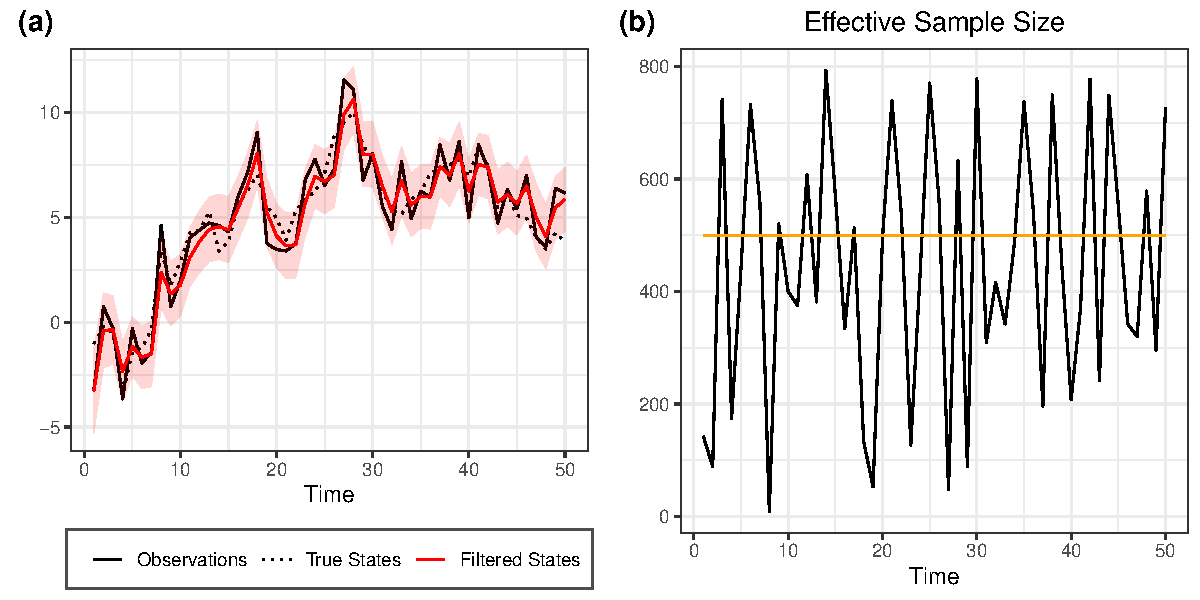
\includegraphics{Exemples-and-Implementations_files/figure-latex/unnamed-chunk-13-1.pdf}

\begin{Shaded}
\begin{Highlighting}[]
\NormalTok{Comparethetwo}\OtherTok{\textless{}{-}}\FunctionTok{matrix}\NormalTok{(}\ConstantTok{NA}\NormalTok{,}\AttributeTok{nrow=}\DecValTok{2}\NormalTok{,}\AttributeTok{ncol=}\DecValTok{2}\NormalTok{)}
\FunctionTok{colnames}\NormalTok{(Comparethetwo)}\OtherTok{\textless{}{-}}\FunctionTok{c}\NormalTok{(}\StringTok{"Coverage"}\NormalTok{,}\StringTok{"RMSE"}\NormalTok{)}
\FunctionTok{rownames}\NormalTok{(Comparethetwo)}\OtherTok{\textless{}{-}}\FunctionTok{c}\NormalTok{(}\StringTok{"transition"}\NormalTok{,}\StringTok{"more efficient"}\NormalTok{)}
\NormalTok{Comparethetwo[}\DecValTok{1}\NormalTok{,}\DecValTok{1}\NormalTok{]}\OtherTok{\textless{}{-}}\FunctionTok{Coverage}\NormalTok{(pf1)}
\NormalTok{Comparethetwo[}\DecValTok{2}\NormalTok{,}\DecValTok{1}\NormalTok{]}\OtherTok{\textless{}{-}}\FunctionTok{Coverage}\NormalTok{(pf2)}
\NormalTok{Comparethetwo[}\DecValTok{1}\NormalTok{,}\DecValTok{2}\NormalTok{]}\OtherTok{\textless{}{-}}\FunctionTok{RMSE}\NormalTok{(truex,}\FunctionTok{Filtervalues}\NormalTok{(pf1)}\SpecialCharTok{$}\NormalTok{mean)}
\NormalTok{Comparethetwo[}\DecValTok{2}\NormalTok{,}\DecValTok{2}\NormalTok{]}\OtherTok{\textless{}{-}}\FunctionTok{RMSE}\NormalTok{(truex,}\FunctionTok{Filtervalues}\NormalTok{(pf2)}\SpecialCharTok{$}\NormalTok{mean)}
\end{Highlighting}
\end{Shaded}

\begin{longtable}[t]{lcc}
\caption{\label{tab:unnamed-chunk-15}Comparison}\\
\toprule
  & Coverage & RMSE\\
\midrule
transition & 0.94 & 0.883\\
more efficient & 0.90 & 0.873\\
\bottomrule
\end{longtable}

\textbf{Guided Particle Filter}

Let's consider another toy example. Suppose that we have the following
model

\begin{Shaded}
\begin{Highlighting}[]
\NormalTok{GPFfun}\OtherTok{\textless{}{-}}\ControlFlowTok{function}\NormalTok{(data,N,m0,C0,tau,sigma,r)\{}
 \ControlFlowTok{if}\NormalTok{(}\FunctionTok{missing}\NormalTok{(r))\{r}\OtherTok{=}\DecValTok{2}\NormalTok{\}}\ControlFlowTok{else}\NormalTok{\{\}}
\NormalTok{   xs}\OtherTok{\textless{}{-}}\ConstantTok{NULL}
\NormalTok{  ws}\OtherTok{\textless{}{-}}\ConstantTok{NULL}
\NormalTok{  ess}\OtherTok{\textless{}{-}}\ConstantTok{NULL}
\NormalTok{  x  }\OtherTok{=} \FunctionTok{rnorm}\NormalTok{(N,m0,}\FunctionTok{sqrt}\NormalTok{(C0))}
\NormalTok{  w  }\OtherTok{=} \FunctionTok{rep}\NormalTok{(}\DecValTok{1}\SpecialCharTok{/}\NormalTok{N,N)}
  
  \ControlFlowTok{for}\NormalTok{(t }\ControlFlowTok{in} \DecValTok{1}\SpecialCharTok{:}\FunctionTok{length}\NormalTok{(data))\{}
    
\NormalTok{    xprev}\OtherTok{\textless{}{-}}\NormalTok{x}
\NormalTok{    x}\OtherTok{\textless{}{-}}\FunctionTok{rnorm}\NormalTok{(N,x,tau)}
\NormalTok{    w1}\OtherTok{\textless{}{-}}\NormalTok{w}\SpecialCharTok{*}\FunctionTok{dnorm}\NormalTok{(data[t],x,sigma)}\SpecialCharTok{*}\FunctionTok{dnorm}\NormalTok{(x,xprev,tau)}\SpecialCharTok{*}\FunctionTok{I}\NormalTok{(x}\SpecialCharTok{\textgreater{}}\DecValTok{0}\NormalTok{)}\SpecialCharTok{/}\FunctionTok{dnorm}\NormalTok{(x,xprev,tau)}
    
\NormalTok{    w }\OtherTok{=}\NormalTok{ w1}\SpecialCharTok{/}\FunctionTok{sum}\NormalTok{(w1)}
\NormalTok{    ESS  }\OtherTok{=} \DecValTok{1}\SpecialCharTok{/}\FunctionTok{sum}\NormalTok{(w}\SpecialCharTok{\^{}}\DecValTok{2}\NormalTok{)}
    
    \ControlFlowTok{if}\NormalTok{(ESS}\SpecialCharTok{\textless{}}\NormalTok{(N}\SpecialCharTok{/}\NormalTok{r))\{}
\NormalTok{      index}\OtherTok{\textless{}{-}}\FunctionTok{sample}\NormalTok{(N,}\AttributeTok{size=}\NormalTok{N,}\AttributeTok{replace=}\NormalTok{T,}\AttributeTok{prob=}\NormalTok{w)}
\NormalTok{      x}\OtherTok{\textless{}{-}}\NormalTok{x[index]}
\NormalTok{      w}\OtherTok{\textless{}{-}}\FunctionTok{rep}\NormalTok{(}\DecValTok{1}\SpecialCharTok{/}\NormalTok{N,N)}
\NormalTok{    \}}\ControlFlowTok{else}\NormalTok{\{\}}
    
\NormalTok{    xs }\OtherTok{=} \FunctionTok{rbind}\NormalTok{(xs,x)}
\NormalTok{    ws }\OtherTok{=} \FunctionTok{rbind}\NormalTok{(ws,w)}
\NormalTok{    ess }\OtherTok{=}\FunctionTok{rbind}\NormalTok{(ess,ESS)}
\NormalTok{  \}}
  \FunctionTok{return}\NormalTok{(}\FunctionTok{list}\NormalTok{(}\AttributeTok{xs=}\NormalTok{xs,}\AttributeTok{ws=}\NormalTok{ws,}\AttributeTok{ess=}\NormalTok{ess))}
\NormalTok{\}}
\end{Highlighting}
\end{Shaded}

\textbf{}

With reference to the linear gaussian model of section XX, a very basic
auxiliary particle sampling technique is

\begin{itemize}
\item Let $\{(x_{t-1},w_{t-1})^{(i)}\}_{i=1}^{N}$ summarizes $p(x_{t-1}|y_{t-1})$
\end{itemize}

For \(k=1,...,N\)

\begin{itemize}
\item Draw $I_{k}$ with $P(I_{k}) \propto w_{t-1}^{(i)}f(y_{t}|g(x_{t-1}^{(i)})) $ where $g(x_{t-1}^{(i)})=E(X_{t}|X_{t-1})$
\item Draw $x_{t}^{(k)} \sim N(x_{t-1}^{(I_{k})},\tau^2)$
\item Set  $w_{t}^{(k)} = \frac{f_{N}(y_{t}|x_{t}^{(k)})}{f_{N}(y_{t}|g(x_{t-1}^{(I_{k})}))}$
\end{itemize}

The remaining steps are the same of the particle filter already seen in
section XX.

\begin{Shaded}
\begin{Highlighting}[]
\NormalTok{APFfun}\OtherTok{\textless{}{-}}\ControlFlowTok{function}\NormalTok{(data,N,m0,C0,tau,sigma,r)\{}
  \ControlFlowTok{if}\NormalTok{(}\FunctionTok{missing}\NormalTok{(r))\{r}\OtherTok{=}\DecValTok{2}\NormalTok{\}}\ControlFlowTok{else}\NormalTok{\{\}}
\NormalTok{  xs}\OtherTok{\textless{}{-}}\ConstantTok{NULL}
\NormalTok{  ws}\OtherTok{\textless{}{-}}\ConstantTok{NULL}
\NormalTok{  ess}\OtherTok{\textless{}{-}}\ConstantTok{NULL}
\NormalTok{  x  }\OtherTok{=} \FunctionTok{rnorm}\NormalTok{(N,m0,}\FunctionTok{sqrt}\NormalTok{(C0))}
\NormalTok{  w  }\OtherTok{=} \FunctionTok{rep}\NormalTok{(}\DecValTok{1}\SpecialCharTok{/}\NormalTok{N,N)}
  
  \ControlFlowTok{for}\NormalTok{(t }\ControlFlowTok{in} \DecValTok{1}\SpecialCharTok{:}\FunctionTok{length}\NormalTok{(data))\{}
    
\NormalTok{    weight }\OtherTok{=}\NormalTok{ w}\SpecialCharTok{*}\FunctionTok{dnorm}\NormalTok{(data[t],x,sigma)}
\NormalTok{    k   }\OtherTok{=} \FunctionTok{sample}\NormalTok{(}\DecValTok{1}\SpecialCharTok{:}\NormalTok{N,}\AttributeTok{size=}\NormalTok{N,}\AttributeTok{replace=}\ConstantTok{TRUE}\NormalTok{,}\AttributeTok{prob=}\NormalTok{weight)}
\NormalTok{    x1   }\OtherTok{=} \FunctionTok{rnorm}\NormalTok{(N,x[k],tau)}
\NormalTok{    lw  }\OtherTok{=} \FunctionTok{dnorm}\NormalTok{(data[t],x1,sigma,}\AttributeTok{log=}\ConstantTok{TRUE}\NormalTok{)}\SpecialCharTok{{-}}\FunctionTok{dnorm}\NormalTok{(data[t],x[k],sigma,}\AttributeTok{log=}\ConstantTok{TRUE}\NormalTok{)}
\NormalTok{    w   }\OtherTok{=} \FunctionTok{exp}\NormalTok{(lw)}
\NormalTok{    w   }\OtherTok{=}\NormalTok{ w}\SpecialCharTok{/}\FunctionTok{sum}\NormalTok{(w)}
\NormalTok{    ESS  }\OtherTok{=} \DecValTok{1}\SpecialCharTok{/}\FunctionTok{sum}\NormalTok{(w}\SpecialCharTok{\^{}}\DecValTok{2}\NormalTok{)}
    
    \ControlFlowTok{if}\NormalTok{(ESS}\SpecialCharTok{\textless{}}\NormalTok{(N}\SpecialCharTok{/}\NormalTok{r))\{}
\NormalTok{      index}\OtherTok{\textless{}{-}}\FunctionTok{sample}\NormalTok{(N,}\AttributeTok{size=}\NormalTok{N,}\AttributeTok{replace=}\NormalTok{T,}\AttributeTok{prob=}\NormalTok{w)}
\NormalTok{      x1}\OtherTok{\textless{}{-}}\NormalTok{x1[index]}
\NormalTok{      w}\OtherTok{\textless{}{-}}\FunctionTok{rep}\NormalTok{(}\DecValTok{1}\SpecialCharTok{/}\NormalTok{N,N)}
\NormalTok{    \}}\ControlFlowTok{else}\NormalTok{\{\}}
    
\NormalTok{    x }\OtherTok{\textless{}{-}}\NormalTok{ x1}
\NormalTok{    xs }\OtherTok{=} \FunctionTok{rbind}\NormalTok{(xs,x)}
\NormalTok{    ws }\OtherTok{=} \FunctionTok{rbind}\NormalTok{(ws,w)}
\NormalTok{    ess }\OtherTok{=}\FunctionTok{rbind}\NormalTok{(ess,ESS)}
    
\NormalTok{  \}}
  \FunctionTok{return}\NormalTok{(}\FunctionTok{list}\NormalTok{(}\AttributeTok{xs=}\NormalTok{xs,}\AttributeTok{ws=}\NormalTok{ws,}\AttributeTok{ess=}\NormalTok{ess))}
\NormalTok{\}}
\end{Highlighting}
\end{Shaded}

\includegraphics{Exemples-and-Implementations_files/figure-latex/unnamed-chunk-18-1.pdf}

\begin{figure}[ht]

{\centering 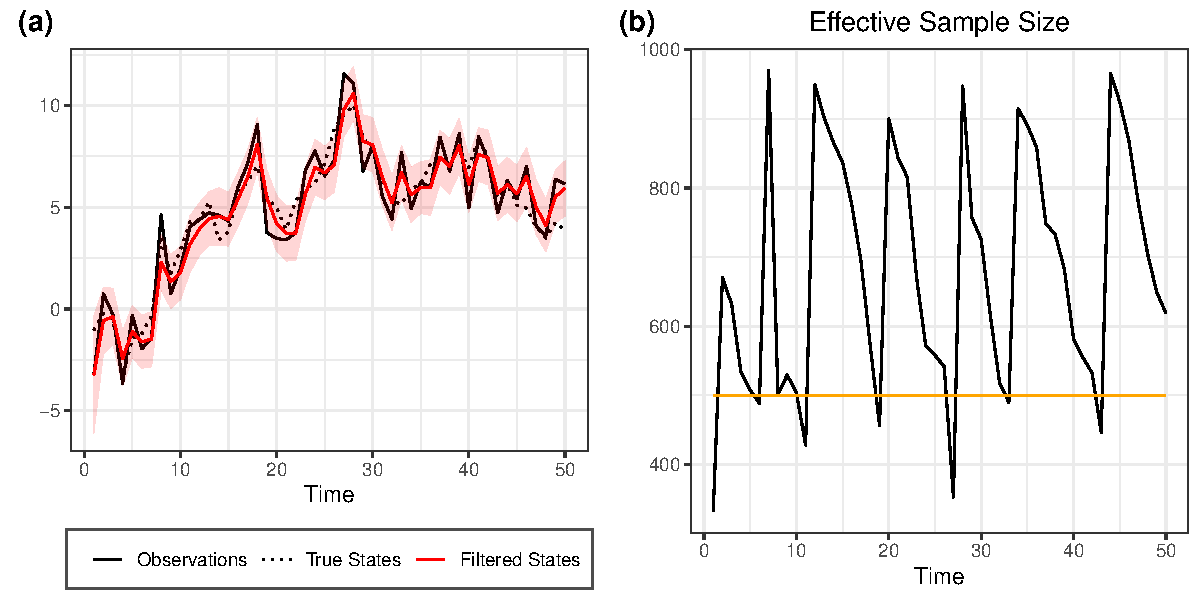
\includegraphics{Exemples-and-Implementations_files/figure-latex/unnamed-chunk-19-1} 

}

\caption{Particle Filtered States with credible interval (in red)}\label{fig:unnamed-chunk-19}
\end{figure}

\hfill\break
\textbf{Liu and West Filter}\\
Consider the toy example of section XX. Let
\(\psi=(\sigma^{2},\tau^{2})\) be unknown and assign a gamma prior on
these parameters \begin{align*}
\sigma^{2}  & \sim G(\alpha_{v},\beta_{v}) \\
\tau^{2}  & \sim G(\alpha_{w},\beta_{w})
\end{align*} or let assign them a uniform prior if we have no knowledge
on hyperparameters. After having drown the hyperparameters indipendently
form their priors and having set \(w_{0}^{(i)}=N^{-1}\), \(i=1,...,N\),
and
\(\hat{\pi}_{0}=\sum_{i=1}^{N}w_{0}^{(i)}\delta_{(x_{0}^{(i)},\psi^{(i)})}\),
for t=1,..T

\begin{itemize}
\item Compute $\hat{\psi}=E_{\hat{\pi}_{t-1}}(\psi)$ and $\Sigma=Var_{\hat{\pi}_{t-1}}(\psi)$. For $i=1,...,N$ set
\begin{align*}
m(\psi^{(i)}) & =a\psi^{(i)}+(1-a)\overline{\psi}\\
v(\psi^{(i)}) & =(1-a^2)\Sigma
\end{align*}
and
\begin{align*}
\alpha(\psi^{(i)}) & =\frac{m(\psi^{(i)})^2}{v(\psi^{(i)})} \\
\beta(\psi^{(i)}) & =\frac{m(\psi^{(i)})}{v(\psi^{(i)})}
\end{align*}
For $k=1,...,N$
\begin{itemize}
\item Draw $I_{k}$ with $P(I_{k}=i) \propto w_{t-1^{(i)}}f_{N}(y_{t}|g(x_{t}^{(i)}),m(\psi^{(i)}))$ where for simplicity $g(x_{t}^{(i)})=E(x_{t}|x_{t-1},m(\psi^{(i)}))$
\item Draw $\psi^{(k)} \sim G(\alpha(\psi^{(I_{k})}),\beta(\psi^{(I_{k})}))$
\item Draw $x_{t}^{(k)} \sim N(x_{t-1}^{(I_{k})},\tau^{{2}^{(k)}})$
\item Set $\tilde{w}_{t}^{k}=\frac{f_N(y_{t}|x_{t}^{(k)},\psi=\psi^{(k)})}{f_N(y_{t}|g(x_{t}^{(I_{k})}),\psi=m(\psi)^{(I_k)})}$
\end{itemize}
\item Normalize the weights
\item Compute the effective sample size ($ESS$)
\item If $ESS<N/2$, resample:
\begin{itemize}
\item Draw a sample of size N, $x_{t}^{(1)},...,x_{t}^{(N)}$,from the discrete distribution $P((x_{t},\psi)=(x_{t}^{(i)},\psi^{(i)}))=w_{t}^{(i)},\ \ i=1,...,N$
\item Reset the weights: $w_{t}^{(i)}=N^{-1}$, $i=1,...,N$.
\end{itemize}

\end{itemize}

\begin{Shaded}
\begin{Highlighting}[]
\NormalTok{LWfun}\OtherTok{\textless{}{-}}\ControlFlowTok{function}\NormalTok{(data,N,m0,C0,alphav,betav,alphaw,betaw,delta,unif,r)\{}
  \ControlFlowTok{if}\NormalTok{(}\FunctionTok{missing}\NormalTok{(r))\{r}\OtherTok{=}\DecValTok{2}\NormalTok{\}}\ControlFlowTok{else}\NormalTok{\{\}}
\NormalTok{  xs     }\OtherTok{=} \FunctionTok{rnorm}\NormalTok{(N,m0,}\FunctionTok{sqrt}\NormalTok{(C0))}
  \ControlFlowTok{if}\NormalTok{(unif}\SpecialCharTok{==}\NormalTok{T)\{}
\NormalTok{  pars   }\OtherTok{=} \FunctionTok{cbind}\NormalTok{(}\FunctionTok{runif}\NormalTok{(N,}\DecValTok{0}\NormalTok{,}\DecValTok{10}\NormalTok{),}\FunctionTok{runif}\NormalTok{(N,}\DecValTok{0}\NormalTok{,}\DecValTok{10}\NormalTok{))\}}\ControlFlowTok{else}\NormalTok{\{\}}
\NormalTok{  pars   }\OtherTok{=} \FunctionTok{cbind}\NormalTok{(}\FunctionTok{rgamma}\NormalTok{(N,}\AttributeTok{shape=}\NormalTok{alphav,}\AttributeTok{scale=}\NormalTok{betav),}\FunctionTok{rgamma}\NormalTok{(N,}\AttributeTok{shape=}\NormalTok{alphaw,}\AttributeTok{scale=}\NormalTok{betaw))}
\NormalTok{  a      }\OtherTok{=}\NormalTok{ (}\DecValTok{3}\SpecialCharTok{*}\NormalTok{delta}\DecValTok{{-}1}\NormalTok{)}\SpecialCharTok{/}\NormalTok{(}\DecValTok{2}\SpecialCharTok{*}\NormalTok{delta)}
\NormalTok{  h2     }\OtherTok{=} \DecValTok{1}\SpecialCharTok{{-}}\NormalTok{a}\SpecialCharTok{\^{}}\DecValTok{2}
\NormalTok{  parss  }\OtherTok{=} \FunctionTok{array}\NormalTok{(}\DecValTok{0}\NormalTok{,}\FunctionTok{c}\NormalTok{(N,}\DecValTok{2}\NormalTok{,n))}
\NormalTok{  xss    }\OtherTok{=} \ConstantTok{NULL}
\NormalTok{  ws     }\OtherTok{=} \ConstantTok{NULL}
\NormalTok{  ess    }\OtherTok{=} \ConstantTok{NULL}
\NormalTok{  w      }\OtherTok{=} \FunctionTok{rep}\NormalTok{(}\DecValTok{1}\SpecialCharTok{/}\NormalTok{N,N)}
  \ControlFlowTok{for}\NormalTok{ (t }\ControlFlowTok{in} \DecValTok{1}\SpecialCharTok{:}\FunctionTok{length}\NormalTok{(data))\{}
\NormalTok{    meanV }\OtherTok{=} \FunctionTok{weighted.mean}\NormalTok{(pars[,}\DecValTok{1}\NormalTok{],w)}
\NormalTok{    varV  }\OtherTok{=} \FunctionTok{weighted.mean}\NormalTok{((pars[,}\DecValTok{1}\NormalTok{]}\SpecialCharTok{{-}}\NormalTok{meanV)}\SpecialCharTok{\^{}}\DecValTok{2}\NormalTok{,w)}
\NormalTok{    meanW }\OtherTok{=} \FunctionTok{weighted.mean}\NormalTok{(pars[,}\DecValTok{2}\NormalTok{],w)}
\NormalTok{    varW  }\OtherTok{=} \FunctionTok{weighted.mean}\NormalTok{((pars[,}\DecValTok{2}\NormalTok{]}\SpecialCharTok{{-}}\NormalTok{meanW)}\SpecialCharTok{\^{}}\DecValTok{2}\NormalTok{,w)}
    
\NormalTok{    muV }\OtherTok{=}\NormalTok{ a}\SpecialCharTok{*}\NormalTok{pars[,}\DecValTok{1}\NormalTok{]}\SpecialCharTok{+}\NormalTok{(}\DecValTok{1}\SpecialCharTok{{-}}\NormalTok{a)}\SpecialCharTok{*}\NormalTok{meanV}
\NormalTok{    sigma2V }\OtherTok{=}\NormalTok{ (}\DecValTok{1}\SpecialCharTok{{-}}\NormalTok{a}\SpecialCharTok{\^{}}\DecValTok{2}\NormalTok{)}\SpecialCharTok{*}\NormalTok{varV}
\NormalTok{    alphaV }\OtherTok{=}\NormalTok{ muV}\SpecialCharTok{\^{}}\DecValTok{2}\SpecialCharTok{/}\NormalTok{sigma2V}
\NormalTok{    betaV }\OtherTok{=}\NormalTok{ muV}\SpecialCharTok{/}\NormalTok{sigma2V}
    
\NormalTok{    muW }\OtherTok{=}\NormalTok{ a}\SpecialCharTok{*}\NormalTok{pars[,}\DecValTok{1}\NormalTok{]}\SpecialCharTok{+}\NormalTok{(}\DecValTok{1}\SpecialCharTok{{-}}\NormalTok{a)}\SpecialCharTok{*}\NormalTok{meanW}
\NormalTok{    sigma2W }\OtherTok{=}\NormalTok{ (}\DecValTok{1}\SpecialCharTok{{-}}\NormalTok{a}\SpecialCharTok{\^{}}\DecValTok{2}\NormalTok{)}\SpecialCharTok{*}\NormalTok{varW}
\NormalTok{    alphaW }\OtherTok{=}\NormalTok{ muW}\SpecialCharTok{\^{}}\DecValTok{2}\SpecialCharTok{/}\NormalTok{sigma2W}
\NormalTok{    betaW }\OtherTok{=}\NormalTok{ muW}\SpecialCharTok{/}\NormalTok{sigma2W}
    
\NormalTok{    weight      }\OtherTok{=}\NormalTok{ w}\SpecialCharTok{*}\FunctionTok{dnorm}\NormalTok{(data[t],xs,}\FunctionTok{sqrt}\NormalTok{(muV))}
\NormalTok{    k           }\OtherTok{=} \FunctionTok{sample}\NormalTok{(}\DecValTok{1}\SpecialCharTok{:}\NormalTok{N,}\AttributeTok{size=}\NormalTok{N,}\AttributeTok{replace=}\NormalTok{T,}\AttributeTok{prob=}\NormalTok{weight)}
    
\NormalTok{    pars[,}\DecValTok{1}\NormalTok{]}\OtherTok{\textless{}{-}}\FunctionTok{rgamma}\NormalTok{(N,}\AttributeTok{shape=}\NormalTok{alphaV[k],}\AttributeTok{rate=}\NormalTok{betaV[k])}
\NormalTok{    pars[,}\DecValTok{2}\NormalTok{]}\OtherTok{\textless{}{-}}\FunctionTok{rgamma}\NormalTok{(N,}\AttributeTok{shape=}\NormalTok{alphaW[k],}\AttributeTok{rate=}\NormalTok{betaW[k])}
    
\NormalTok{    xsprevious}\OtherTok{\textless{}{-}}\NormalTok{xs[k]}
\NormalTok{    xs }\OtherTok{=} \FunctionTok{rnorm}\NormalTok{(N,xs[k],}\FunctionTok{sqrt}\NormalTok{(pars[,}\DecValTok{2}\NormalTok{]))}
    
\NormalTok{    w           }\OtherTok{=} \FunctionTok{exp}\NormalTok{(}\FunctionTok{dnorm}\NormalTok{( data[t],xs,}\FunctionTok{sqrt}\NormalTok{(pars[,}\DecValTok{1}\NormalTok{]),}\AttributeTok{log=}\NormalTok{T)}\SpecialCharTok{{-}}
                        \FunctionTok{dnorm}\NormalTok{( data[t],xsprevious,}\FunctionTok{sqrt}\NormalTok{(muV[k]),}\AttributeTok{log=}\NormalTok{T))}
\NormalTok{    w           }\OtherTok{=}\NormalTok{ w}\SpecialCharTok{/}\FunctionTok{sum}\NormalTok{(w)}
\NormalTok{    ESS         }\OtherTok{=} \DecValTok{1}\SpecialCharTok{/}\FunctionTok{sum}\NormalTok{(w}\SpecialCharTok{\^{}}\DecValTok{2}\NormalTok{)}
    
    \ControlFlowTok{if}\NormalTok{(ESS}\SpecialCharTok{\textless{}}\NormalTok{(N}\SpecialCharTok{/}\NormalTok{r))\{}
\NormalTok{      index}\OtherTok{\textless{}{-}}\FunctionTok{sample}\NormalTok{(N,}\AttributeTok{size=}\NormalTok{N,}\AttributeTok{replace=}\NormalTok{T,}\AttributeTok{prob=}\NormalTok{w)}
\NormalTok{      xs}\OtherTok{\textless{}{-}}\NormalTok{xs[index]}
\NormalTok{      pars}\OtherTok{\textless{}{-}}\NormalTok{pars[index,]}
\NormalTok{      w}\OtherTok{\textless{}{-}}\FunctionTok{rep}\NormalTok{(}\DecValTok{1}\SpecialCharTok{/}\NormalTok{N,N)}
\NormalTok{    \}}\ControlFlowTok{else}\NormalTok{\{}
\NormalTok{      xs}\OtherTok{\textless{}{-}}\NormalTok{xs}
\NormalTok{      pars}\OtherTok{\textless{}{-}}\NormalTok{pars}
\NormalTok{    \}}
    
    
\NormalTok{    xss         }\OtherTok{=} \FunctionTok{rbind}\NormalTok{(xss,xs)}
\NormalTok{    parss[,,t]  }\OtherTok{=}\NormalTok{ pars }
\NormalTok{    ws          }\OtherTok{=} \FunctionTok{rbind}\NormalTok{(ws,w)}
\NormalTok{    ess         }\OtherTok{=} \FunctionTok{rbind}\NormalTok{(ess,ESS)}
\NormalTok{  \}}
  \FunctionTok{return}\NormalTok{(}\FunctionTok{list}\NormalTok{(}\AttributeTok{xss=}\NormalTok{xss,}\AttributeTok{parss=}\NormalTok{parss,}\AttributeTok{ws=}\NormalTok{ws,}\AttributeTok{ess=}\NormalTok{ess))}
\NormalTok{\}}
\end{Highlighting}
\end{Shaded}

\includegraphics{Exemples-and-Implementations_files/figure-latex/unnamed-chunk-21-1.pdf}

\begin{figure}[ht]

{\centering 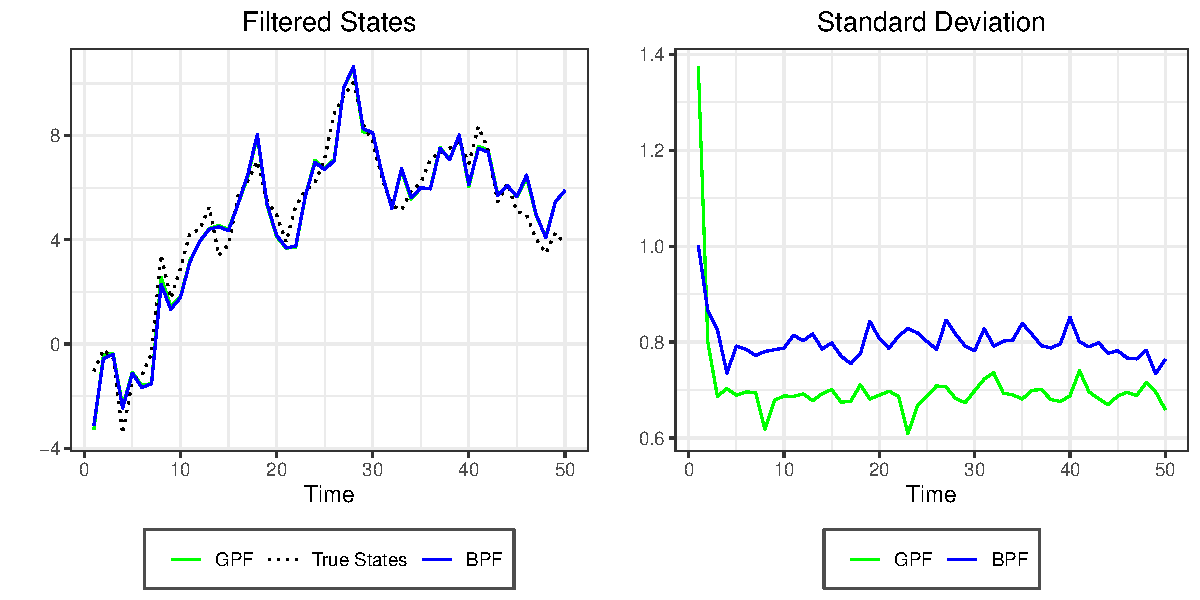
\includegraphics{Exemples-and-Implementations_files/figure-latex/unnamed-chunk-22-1} 

}

\caption{Particle Filtered States with credible interval (in red)}\label{fig:unnamed-chunk-22}
\end{figure}

\hypertarget{comparison-another-section}{%
\section{COMPARISON (ANOTHER
SECTION)}\label{comparison-another-section}}

\begin{figure}[ht]

{\centering 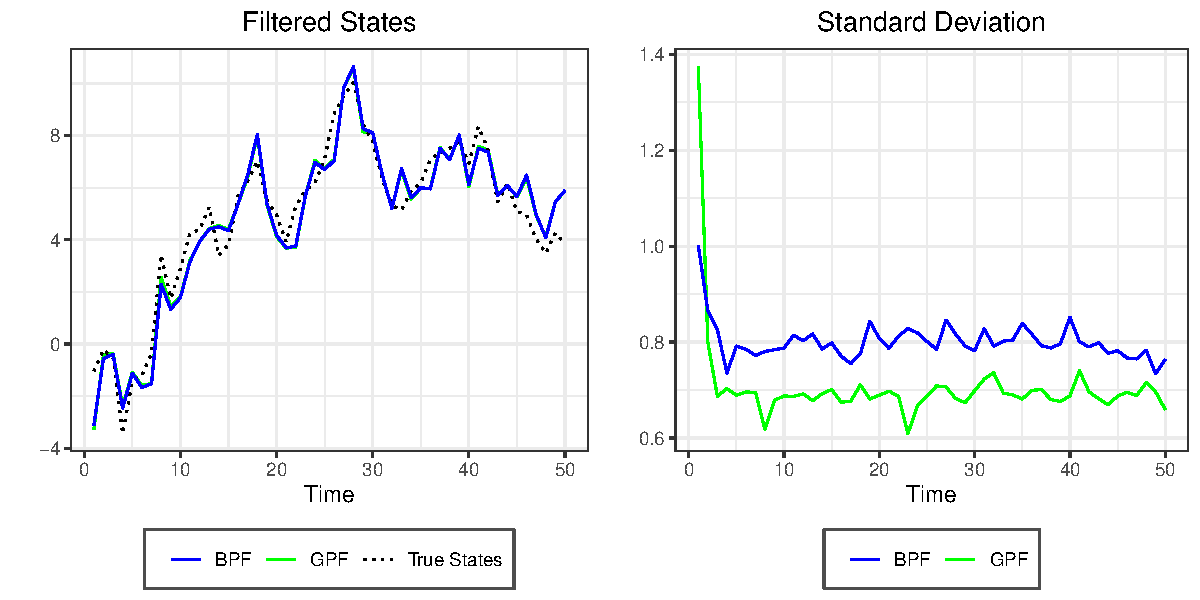
\includegraphics{Exemples-and-Implementations_files/figure-latex/unnamed-chunk-23-1} 

}

\caption{Variances}\label{fig:unnamed-chunk-23}
\end{figure}

\begin{longtable}[t]{cccccc}
\caption{\label{tab:unnamed-chunk-25}RMSE}\\
\toprule
N & Threshold & KF & PF & APF & LWF\\
\midrule
20 & 0.5 & 0.879 & 0.837 & 0.905 & 0.925\\
100 & 0.5 & 0.879 & 0.877 & 0.863 & 0.893\\
500 & 0.5 & 0.879 & 0.881 & 0.889 & 0.882\\
\bottomrule
\end{longtable}

\begin{longtable}[t]{cccccc}
\caption{\label{tab:unnamed-chunk-26}RMSE}\\
\toprule
N & Threshold & KF & PF & APF & LWF\\
\midrule
1000 & 0.50 & 0.879 & 0.911 & 0.877 & 0.884\\
1000 & 0.25 & 0.879 & 0.881 & 0.858 & 0.910\\
1000 & 0.10 & 0.879 & 0.858 & 0.881 & 0.896\\
\bottomrule
\end{longtable}

\hypertarget{stochastic-volatility}{%
\section{STOCHASTIC VOLATILITY}\label{stochastic-volatility}}

Basic specification of Stochastic Volatilty Model \begin{align}
y_{t}|x_{t} & \sim N(0,e^{x_{t}}) \\
x_{t}|x_{t-1} & \sim N(\alpha+\beta x_{t-1},\tau^2)
\end{align}\\

\begin{figure}[ht]

{\centering 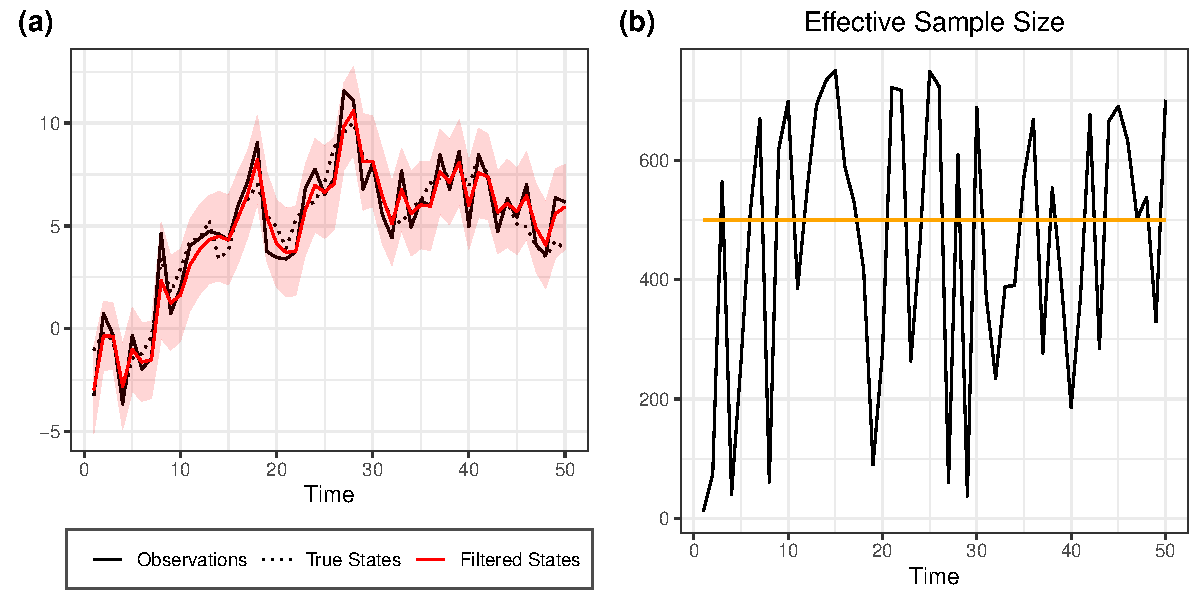
\includegraphics{Exemples-and-Implementations_files/figure-latex/unnamed-chunk-28-1} 

}

\caption{SV}\label{fig:unnamed-chunk-28}
\end{figure}

\textbf{Particle Filter}\\

\begin{Shaded}
\begin{Highlighting}[]
\NormalTok{SVPFfun}\OtherTok{\textless{}{-}}\ControlFlowTok{function}\NormalTok{(data,N,m0,C0,alpha,beta,tau,r)\{}
  \ControlFlowTok{if}\NormalTok{(}\FunctionTok{missing}\NormalTok{(r))\{r}\OtherTok{=}\DecValTok{2}\NormalTok{\}}\ControlFlowTok{else}\NormalTok{\{\}}
\NormalTok{  xs}\OtherTok{\textless{}{-}}\ConstantTok{NULL}
\NormalTok{  ws}\OtherTok{\textless{}{-}}\ConstantTok{NULL}
\NormalTok{  ess}\OtherTok{\textless{}{-}}\ConstantTok{NULL}
\NormalTok{  x  }\OtherTok{=} \FunctionTok{rnorm}\NormalTok{(N,m0,}\FunctionTok{sqrt}\NormalTok{(C0))}
\NormalTok{  w  }\OtherTok{=} \FunctionTok{rep}\NormalTok{(}\DecValTok{1}\SpecialCharTok{/}\NormalTok{N,N)}
   
  \ControlFlowTok{for}\NormalTok{(t }\ControlFlowTok{in} \DecValTok{1}\SpecialCharTok{:}\FunctionTok{length}\NormalTok{(data))\{}
    
\NormalTok{    x}\OtherTok{\textless{}{-}}\FunctionTok{rnorm}\NormalTok{(N,alpha}\SpecialCharTok{+}\NormalTok{beta}\SpecialCharTok{*}\NormalTok{x,tau)}
\NormalTok{    w1}\OtherTok{\textless{}{-}}\NormalTok{w}\SpecialCharTok{*}\FunctionTok{dnorm}\NormalTok{(data[t],}\DecValTok{0}\NormalTok{,}\FunctionTok{exp}\NormalTok{(x}\SpecialCharTok{/}\DecValTok{2}\NormalTok{))}
    
\NormalTok{    w }\OtherTok{=}\NormalTok{ w1}\SpecialCharTok{/}\FunctionTok{sum}\NormalTok{(w1)}
\NormalTok{    ESS  }\OtherTok{=} \DecValTok{1}\SpecialCharTok{/}\FunctionTok{sum}\NormalTok{(w}\SpecialCharTok{\^{}}\DecValTok{2}\NormalTok{)}
    
    \ControlFlowTok{if}\NormalTok{(ESS}\SpecialCharTok{\textless{}}\NormalTok{(N}\SpecialCharTok{/}\NormalTok{r))\{}
\NormalTok{      index}\OtherTok{\textless{}{-}}\FunctionTok{sample}\NormalTok{(N,}\AttributeTok{size=}\NormalTok{N,}\AttributeTok{replace=}\NormalTok{T,}\AttributeTok{prob=}\NormalTok{w)}
\NormalTok{      x}\OtherTok{\textless{}{-}}\NormalTok{x[index]}
\NormalTok{      w}\OtherTok{\textless{}{-}}\FunctionTok{rep}\NormalTok{(}\DecValTok{1}\SpecialCharTok{/}\NormalTok{N,N)}
\NormalTok{    \}}\ControlFlowTok{else}\NormalTok{\{\}}
    
\NormalTok{    xs }\OtherTok{=} \FunctionTok{rbind}\NormalTok{(xs,x)}
\NormalTok{    ws }\OtherTok{=} \FunctionTok{rbind}\NormalTok{(ws,w)}
\NormalTok{    ess }\OtherTok{=}\FunctionTok{rbind}\NormalTok{(ess,ESS)}
\NormalTok{  \}}
  \FunctionTok{return}\NormalTok{(}\FunctionTok{list}\NormalTok{(}\AttributeTok{xs=}\NormalTok{xs,}\AttributeTok{ws=}\NormalTok{ws,}\AttributeTok{ess=}\NormalTok{ess))}
\NormalTok{\}}
\end{Highlighting}
\end{Shaded}

\textbf{Auxiliary Particle Filter}

\begin{Shaded}
\begin{Highlighting}[]
\NormalTok{SVAPFfun}\OtherTok{\textless{}{-}}\ControlFlowTok{function}\NormalTok{(data,N,m0,C0,alpha,beta,tau,r)\{}
  \ControlFlowTok{if}\NormalTok{(}\FunctionTok{missing}\NormalTok{(r))\{r}\OtherTok{=}\DecValTok{2}\NormalTok{\}}\ControlFlowTok{else}\NormalTok{\{\}}
\NormalTok{  xs}\OtherTok{\textless{}{-}}\ConstantTok{NULL}
\NormalTok{  ws}\OtherTok{\textless{}{-}}\ConstantTok{NULL}
\NormalTok{  ess}\OtherTok{\textless{}{-}}\ConstantTok{NULL}
\NormalTok{  x  }\OtherTok{=} \FunctionTok{rnorm}\NormalTok{(N,m0,}\FunctionTok{sqrt}\NormalTok{(C0))}
\NormalTok{  w  }\OtherTok{=} \FunctionTok{rep}\NormalTok{(}\DecValTok{1}\SpecialCharTok{/}\NormalTok{N,N)}
  
  \ControlFlowTok{for}\NormalTok{(t }\ControlFlowTok{in} \DecValTok{1}\SpecialCharTok{:}\FunctionTok{length}\NormalTok{(data))\{}
    
\NormalTok{    weight }\OtherTok{=}\NormalTok{ w}\SpecialCharTok{*}\FunctionTok{dnorm}\NormalTok{(data[t],}\DecValTok{0}\NormalTok{,}\FunctionTok{exp}\NormalTok{(x}\SpecialCharTok{/}\DecValTok{2}\NormalTok{))}
\NormalTok{    k   }\OtherTok{=} \FunctionTok{sample}\NormalTok{(}\DecValTok{1}\SpecialCharTok{:}\NormalTok{N,}\AttributeTok{size=}\NormalTok{N,}\AttributeTok{replace=}\ConstantTok{TRUE}\NormalTok{,}\AttributeTok{prob=}\NormalTok{weight)}
\NormalTok{    x1   }\OtherTok{=} \FunctionTok{rnorm}\NormalTok{(N,alpha}\SpecialCharTok{+}\NormalTok{beta}\SpecialCharTok{*}\NormalTok{x[k],tau)}
\NormalTok{    lw  }\OtherTok{=} \FunctionTok{dnorm}\NormalTok{(data[t],}\DecValTok{0}\NormalTok{,}\FunctionTok{exp}\NormalTok{(x}\SpecialCharTok{/}\DecValTok{2}\NormalTok{),}\AttributeTok{log=}\ConstantTok{TRUE}\NormalTok{)}\SpecialCharTok{{-}}\FunctionTok{dnorm}\NormalTok{(data[t],}\DecValTok{0}\NormalTok{,}\FunctionTok{exp}\NormalTok{(x}\SpecialCharTok{/}\DecValTok{2}\NormalTok{),}\AttributeTok{log=}\ConstantTok{TRUE}\NormalTok{)}
\NormalTok{    w   }\OtherTok{=} \FunctionTok{exp}\NormalTok{(lw)}
\NormalTok{    w   }\OtherTok{=}\NormalTok{ w}\SpecialCharTok{/}\FunctionTok{sum}\NormalTok{(w)}
\NormalTok{    ESS  }\OtherTok{=} \DecValTok{1}\SpecialCharTok{/}\FunctionTok{sum}\NormalTok{(w}\SpecialCharTok{\^{}}\DecValTok{2}\NormalTok{)}
    
    \ControlFlowTok{if}\NormalTok{(ESS}\SpecialCharTok{\textless{}}\NormalTok{(N}\SpecialCharTok{/}\NormalTok{r))\{}
\NormalTok{      index}\OtherTok{\textless{}{-}}\FunctionTok{sample}\NormalTok{(N,}\AttributeTok{size=}\NormalTok{N,}\AttributeTok{replace=}\NormalTok{T,}\AttributeTok{prob=}\NormalTok{w)}
\NormalTok{      x1}\OtherTok{\textless{}{-}}\NormalTok{x1[index]}
\NormalTok{      w}\OtherTok{\textless{}{-}}\FunctionTok{rep}\NormalTok{(}\DecValTok{1}\SpecialCharTok{/}\NormalTok{N,N)}
\NormalTok{    \}}\ControlFlowTok{else}\NormalTok{\{\}}
    
\NormalTok{    x }\OtherTok{\textless{}{-}}\NormalTok{ x1}
\NormalTok{    xs }\OtherTok{=} \FunctionTok{rbind}\NormalTok{(xs,x)}
\NormalTok{    ws }\OtherTok{=} \FunctionTok{rbind}\NormalTok{(ws,w)}
\NormalTok{    ess }\OtherTok{=}\FunctionTok{rbind}\NormalTok{(ess,ESS)}
    
\NormalTok{  \}}
  \FunctionTok{return}\NormalTok{(}\FunctionTok{list}\NormalTok{(}\AttributeTok{xs=}\NormalTok{xs,}\AttributeTok{ws=}\NormalTok{ws,}\AttributeTok{ess=}\NormalTok{ess))}
\NormalTok{\}}
\end{Highlighting}
\end{Shaded}

\textbf{Liu and West}

\begin{Shaded}
\begin{Highlighting}[]
\NormalTok{SVLWfun}\OtherTok{\textless{}{-}}\ControlFlowTok{function}\NormalTok{(data,N,m0,C0,ealpha,valpha,ebeta,vbeta,nu,lambda)\{}

\NormalTok{xs }\OtherTok{=} \FunctionTok{rnorm}\NormalTok{(N,m0,}\FunctionTok{sqrt}\NormalTok{(C0))}
\NormalTok{pars   }\OtherTok{=} \FunctionTok{cbind}\NormalTok{(}\FunctionTok{rnorm}\NormalTok{(N,ealpha,}\FunctionTok{sqrt}\NormalTok{(valpha)),}\FunctionTok{rnorm}\NormalTok{(N,ebeta,}\FunctionTok{sqrt}\NormalTok{(vbeta)),}
               \FunctionTok{log}\NormalTok{(}\DecValTok{1}\SpecialCharTok{/}\FunctionTok{rgamma}\NormalTok{(N,nu}\SpecialCharTok{/}\DecValTok{2}\NormalTok{,nu}\SpecialCharTok{*}\NormalTok{lambda}\SpecialCharTok{/}\DecValTok{2}\NormalTok{)))}
\NormalTok{delta  }\OtherTok{=} \FloatTok{0.75}
\NormalTok{a      }\OtherTok{=}\NormalTok{ (}\DecValTok{3}\SpecialCharTok{*}\NormalTok{delta}\DecValTok{{-}1}\NormalTok{)}\SpecialCharTok{/}\NormalTok{(}\DecValTok{2}\SpecialCharTok{*}\NormalTok{delta)}
\NormalTok{h2     }\OtherTok{=} \DecValTok{1}\SpecialCharTok{{-}}\NormalTok{a}\SpecialCharTok{\^{}}\DecValTok{2}
\NormalTok{parss  }\OtherTok{=} \FunctionTok{array}\NormalTok{(}\DecValTok{0}\NormalTok{,}\FunctionTok{c}\NormalTok{(N,}\DecValTok{3}\NormalTok{,n))}
\NormalTok{xss    }\OtherTok{=} \ConstantTok{NULL}
\NormalTok{ws     }\OtherTok{=} \ConstantTok{NULL}
\NormalTok{ESS    }\OtherTok{=} \ConstantTok{NULL}
\NormalTok{w      }\OtherTok{=} \FunctionTok{rep}\NormalTok{(}\DecValTok{1}\SpecialCharTok{/}\NormalTok{N,N)}
\ControlFlowTok{for}\NormalTok{ (t }\ControlFlowTok{in} \DecValTok{1}\SpecialCharTok{:}\FunctionTok{length}\NormalTok{(data))\{}
  
  \CommentTok{\#mpar        = apply(pars,2,mean) \#alternatively use this }
\NormalTok{  mpar}\OtherTok{\textless{}{-}}\FunctionTok{c}\NormalTok{()}
  \ControlFlowTok{for}\NormalTok{(i }\ControlFlowTok{in} \DecValTok{1}\SpecialCharTok{:}\DecValTok{3}\NormalTok{)\{}
\NormalTok{  mpar[i]    }\OtherTok{=} \FunctionTok{weighted.mean}\NormalTok{(pars[,i],w)}
\NormalTok{  \}}
  
\NormalTok{  vpar        }\OtherTok{=} \FunctionTok{var}\NormalTok{(pars)}
\NormalTok{  ms          }\OtherTok{=}\NormalTok{ a}\SpecialCharTok{*}\NormalTok{pars}\SpecialCharTok{+}\NormalTok{(}\DecValTok{1}\SpecialCharTok{{-}}\NormalTok{a)}\SpecialCharTok{*}\FunctionTok{matrix}\NormalTok{(mpar,N,}\DecValTok{3}\NormalTok{,}\AttributeTok{byrow=}\NormalTok{T)}
\NormalTok{  mus         }\OtherTok{=}\NormalTok{ pars[,}\DecValTok{1}\NormalTok{]}\SpecialCharTok{+}\NormalTok{pars[,}\DecValTok{2}\NormalTok{]}\SpecialCharTok{*}\NormalTok{xs }
\NormalTok{  weight      }\OtherTok{=}\NormalTok{ w}\SpecialCharTok{*}\FunctionTok{dnorm}\NormalTok{(data[t],}\DecValTok{0}\NormalTok{,}\FunctionTok{exp}\NormalTok{(mus}\SpecialCharTok{/}\DecValTok{2}\NormalTok{))}
\NormalTok{  k           }\OtherTok{=} \FunctionTok{sample}\NormalTok{(}\DecValTok{1}\SpecialCharTok{:}\NormalTok{N,}\AttributeTok{size=}\NormalTok{N,}\AttributeTok{replace=}\NormalTok{T,}\AttributeTok{prob=}\NormalTok{weight)}
\NormalTok{  ms1         }\OtherTok{=}\NormalTok{ ms[k,] }\SpecialCharTok{+} \FunctionTok{matrix}\NormalTok{(}\FunctionTok{rnorm}\NormalTok{(}\DecValTok{3}\SpecialCharTok{*}\NormalTok{N),N,}\DecValTok{3}\NormalTok{)}\SpecialCharTok{\%*\%}\FunctionTok{chol}\NormalTok{(h2}\SpecialCharTok{*}\NormalTok{vpar)}
\NormalTok{  xt          }\OtherTok{=} \FunctionTok{rnorm}\NormalTok{(N,ms1[,}\DecValTok{1}\NormalTok{]}\SpecialCharTok{+}\NormalTok{ms1[,}\DecValTok{2}\NormalTok{]}\SpecialCharTok{*}\NormalTok{xs[k],}\FunctionTok{exp}\NormalTok{(ms1[,}\DecValTok{3}\NormalTok{]}\SpecialCharTok{/}\DecValTok{2}\NormalTok{))}
\NormalTok{  w           }\OtherTok{=} \FunctionTok{dnorm}\NormalTok{(data[t],}\DecValTok{0}\NormalTok{,}\FunctionTok{exp}\NormalTok{(xt}\SpecialCharTok{/}\DecValTok{2}\NormalTok{))}\SpecialCharTok{/}\FunctionTok{dnorm}\NormalTok{(data[t],}\DecValTok{0}\NormalTok{,}\FunctionTok{exp}\NormalTok{(mus[k]}\SpecialCharTok{/}\DecValTok{2}\NormalTok{))}
\NormalTok{  w           }\OtherTok{=}\NormalTok{ w}\SpecialCharTok{/}\FunctionTok{sum}\NormalTok{(w)}
\NormalTok{  ESS         }\OtherTok{=} \DecValTok{1}\SpecialCharTok{/}\FunctionTok{sum}\NormalTok{(w}\SpecialCharTok{\^{}}\DecValTok{2}\NormalTok{)}
  
  
  \ControlFlowTok{if}\NormalTok{(ESS}\SpecialCharTok{\textless{}}\NormalTok{(N}\SpecialCharTok{/}\DecValTok{2}\NormalTok{))\{}
\NormalTok{    index}\OtherTok{\textless{}{-}}\FunctionTok{sample}\NormalTok{(N,}\AttributeTok{size=}\NormalTok{N,}\AttributeTok{replace=}\NormalTok{T,}\AttributeTok{prob=}\NormalTok{w)}
\NormalTok{    xs}\OtherTok{\textless{}{-}}\NormalTok{xt[index]}
\NormalTok{    pars}\OtherTok{\textless{}{-}}\NormalTok{ms1[index,]}
\NormalTok{    w}\OtherTok{\textless{}{-}}\FunctionTok{rep}\NormalTok{(}\DecValTok{1}\SpecialCharTok{/}\NormalTok{N,N)}
\NormalTok{  \}}\ControlFlowTok{else}\NormalTok{\{}
\NormalTok{    xs}\OtherTok{\textless{}{-}}\NormalTok{xt}
\NormalTok{    pars}\OtherTok{\textless{}{-}}\NormalTok{ms1}
\NormalTok{  \}}
  
\NormalTok{  xss         }\OtherTok{=} \FunctionTok{rbind}\NormalTok{(xss,xs)}
\NormalTok{  parss[,,t]  }\OtherTok{=}\NormalTok{ pars }
\NormalTok{  ws          }\OtherTok{=} \FunctionTok{rbind}\NormalTok{(ws,w)}
\NormalTok{\}}
\FunctionTok{return}\NormalTok{(}\FunctionTok{list}\NormalTok{(}\AttributeTok{xs=}\NormalTok{xss,}\AttributeTok{pars=}\NormalTok{parss,}\AttributeTok{ws=}\NormalTok{ws))}
\NormalTok{\}}
\end{Highlighting}
\end{Shaded}

\begin{figure}[ht]

{\centering 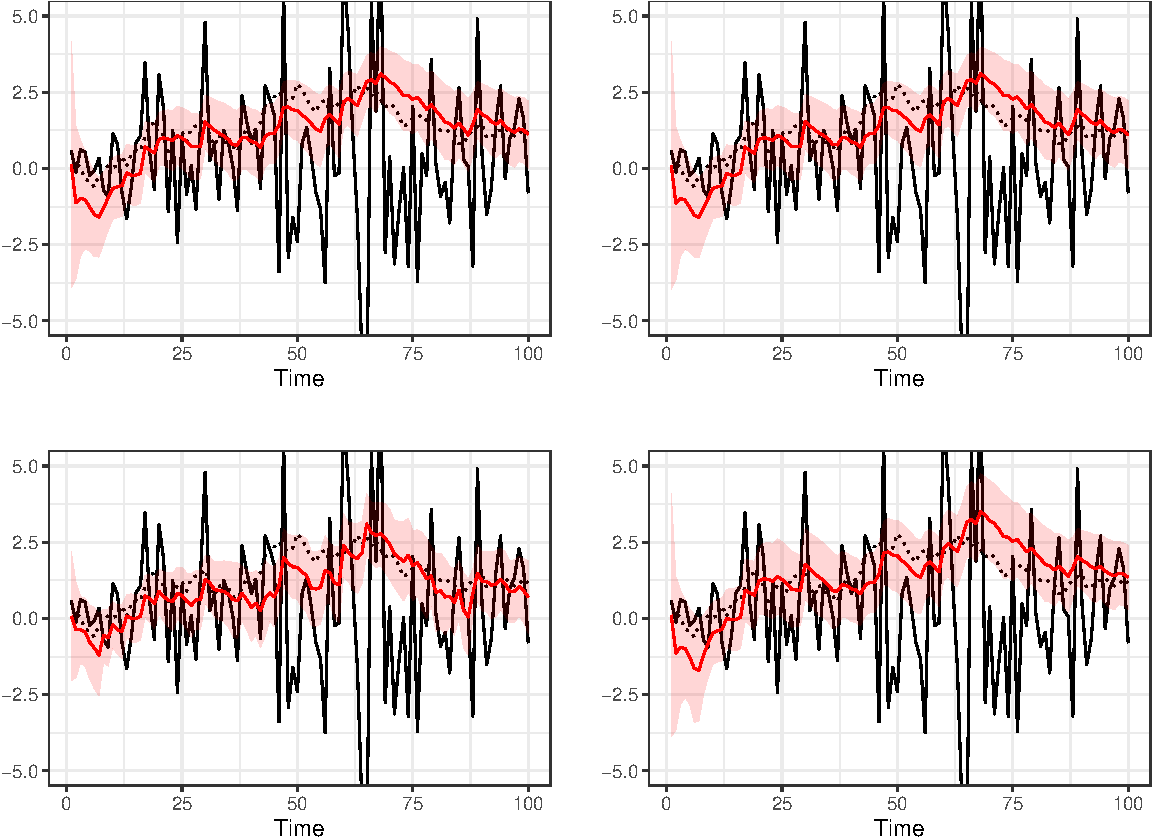
\includegraphics{Exemples-and-Implementations_files/figure-latex/unnamed-chunk-35-1} 

}

\caption{Comparison filter performances}\label{fig:unnamed-chunk-35}
\end{figure}

\end{document}
